The rapid growth of the Electrical Vehicle (EV) market has led to the research of better energy storage.
Lithium-Ion (Li-ion) batteries offer high power density and a low self-discharge rate~\cite{han_review, en13082106}.
Such efficiency made them highly used in the EV application, on top of smartphones or other portable electronic devices.
The misuse of those batteries may lead to rapid battery life degradation (aging) and damage to a device on a small scale or environmental catastrophes in big.
The only solution to an inefficiently used aged battery is recycling and replacement, increasing the usage cost~\cite{skeete_beyond_2020}.
That is why the vital requirement for EV powered with Li-ion batteries is the safe and efficient operation of the integrated Battery Management System (BMS).

%
%
In the BMS application, State of Charge became an issue of great importance.
Since one of the properties of a manufactured Li-ion battery is internal resistance, the voltage reading over a cell becomes unreliable during unstable discharge.
During a system operation process, the voltage drop leads to inaccurate voltage and temperature sensor reading.
Since the depletion of a battery until it cannot supply enough current is undesirable for more prolonged usages, it is crucial to implement a solution to overcome such issues.
A simple battery model that accumulates the multiple of an ideal internal resistance and current consumed by a system became a commonly used solution.
Due to battery aging over longer used, the internal resistance diversifies due to varying battery utilised temperatures.
Eventually, such a simple battery model becomes inefficient and only leads to failure~\cite{fenrg.2019.00065}.
Working temperature, stored charge and maximum output current became different from a freshly manufactured cell.
Therefore, failure to prevent overrated usage lead to battery damage and waisting cell potential earlier than anticipated by manufacturers.
The solution is to use the State of Charge (SoC) as a battery state reference.

%
%
Several methods have been used to make an accurate estimation.
The most commonly used and simple to implement is the Coulomb Counter (CC), integral of the current over time.
However, besides the limitation of not telling the initial SoC, it cannot converge to the actual State of Charge over more prolonged usages~\cite{ng_enhanced_2009}.
The reason for that is the method itself.
The CC model does not consider variations in the battery properties due to degradation, reporting charge percentage by a scale from the first usage.
% \textcolor{red}{(Several other studies if I want to reference them).}
Multiple different and more complicated methods approach this problem in a chemical or complex modelling way.
The methods which will be closer explored in this work are based on statistical Neural Network models.

%
%
In recent years, there have been few different approaches in Artificial Intelligence development for a battery charge estimation: Fuzzy logic, Support Vector Machine, Recurrent Neural Network (RNN).
The RNNs are more commonly used due to their various applications, support from different developers, and being widely tested by researchers.
There have been multiple publications around extensively used Time-Series models, such as Long short-term memory (LSTM) or Gated recurrent units (GRU), for battery state of charge prediction.
\textcolor{red}{A previously published paper of this research [Sadykov, 1] analysed multiple different implementations of RNN models to determine the State of Charge from sensory data like Voltage, Current and Temperature.}
The research results have concluded that sensory data in one behaviour of driving is efficient to estimate but may fall under another.
Thus, the battery state became a matter of not the battery itself but the way it has been used.
Besides, the SoC can fail under-voltage drop under some scenarios, although not as significant and only at certain rate conditions.
The potential solution to the problem was integrating SoC as one of the input features to a NN model.
The limitation here is to be able to get the State of Charge in real-time.
There are two approaches to that, use Charge estimation from other means, CC or three feature-based NN methods, or using the Feed-Forward method to propagate the output value of the charge as an input into the next prediction.

%
%
In this paper, the Long short-term memory model will implement a 4-feature estimator, with a history of 5 to 10 minutes usage, to predict the current State of Charge and propagate the result further.
A novel method of the training loop model will be proposed to eliminate the possibility of accumulating error along with the value of a charge.
It utilises the Autoregressive technique to introduce an adaptive and robust solution to training output inaccuracy over time.
%It meant to force the model to consider the potential of having variations in State of Charge history and yet not fail the prediction output further.
Furthermore, the model is forced to consider a miss accuracy of its State of Charge prediction before loss calculation.

%
%
This paper is organised as follows: a methodology for an RNN model discussed in Section 2.
The details of how auto-regression has been utilised in Section 3.
Subsections 4.1 and 4.2 separates points of model validation and process of parameters estimation.
Finally, section 5 concludes the research along with outlining several observations, which may require separate consideration.
% Most were isolated to closed scenarios with provided data or from battery cycling machine.
% The most promessing approches to improve a model and make it more universal is to increase complexity. While some introduced deeper layer newtwork, others added additional mechanisms to already used.
\begin{landscape}
    \begin{figure}[ht]
        \centering
        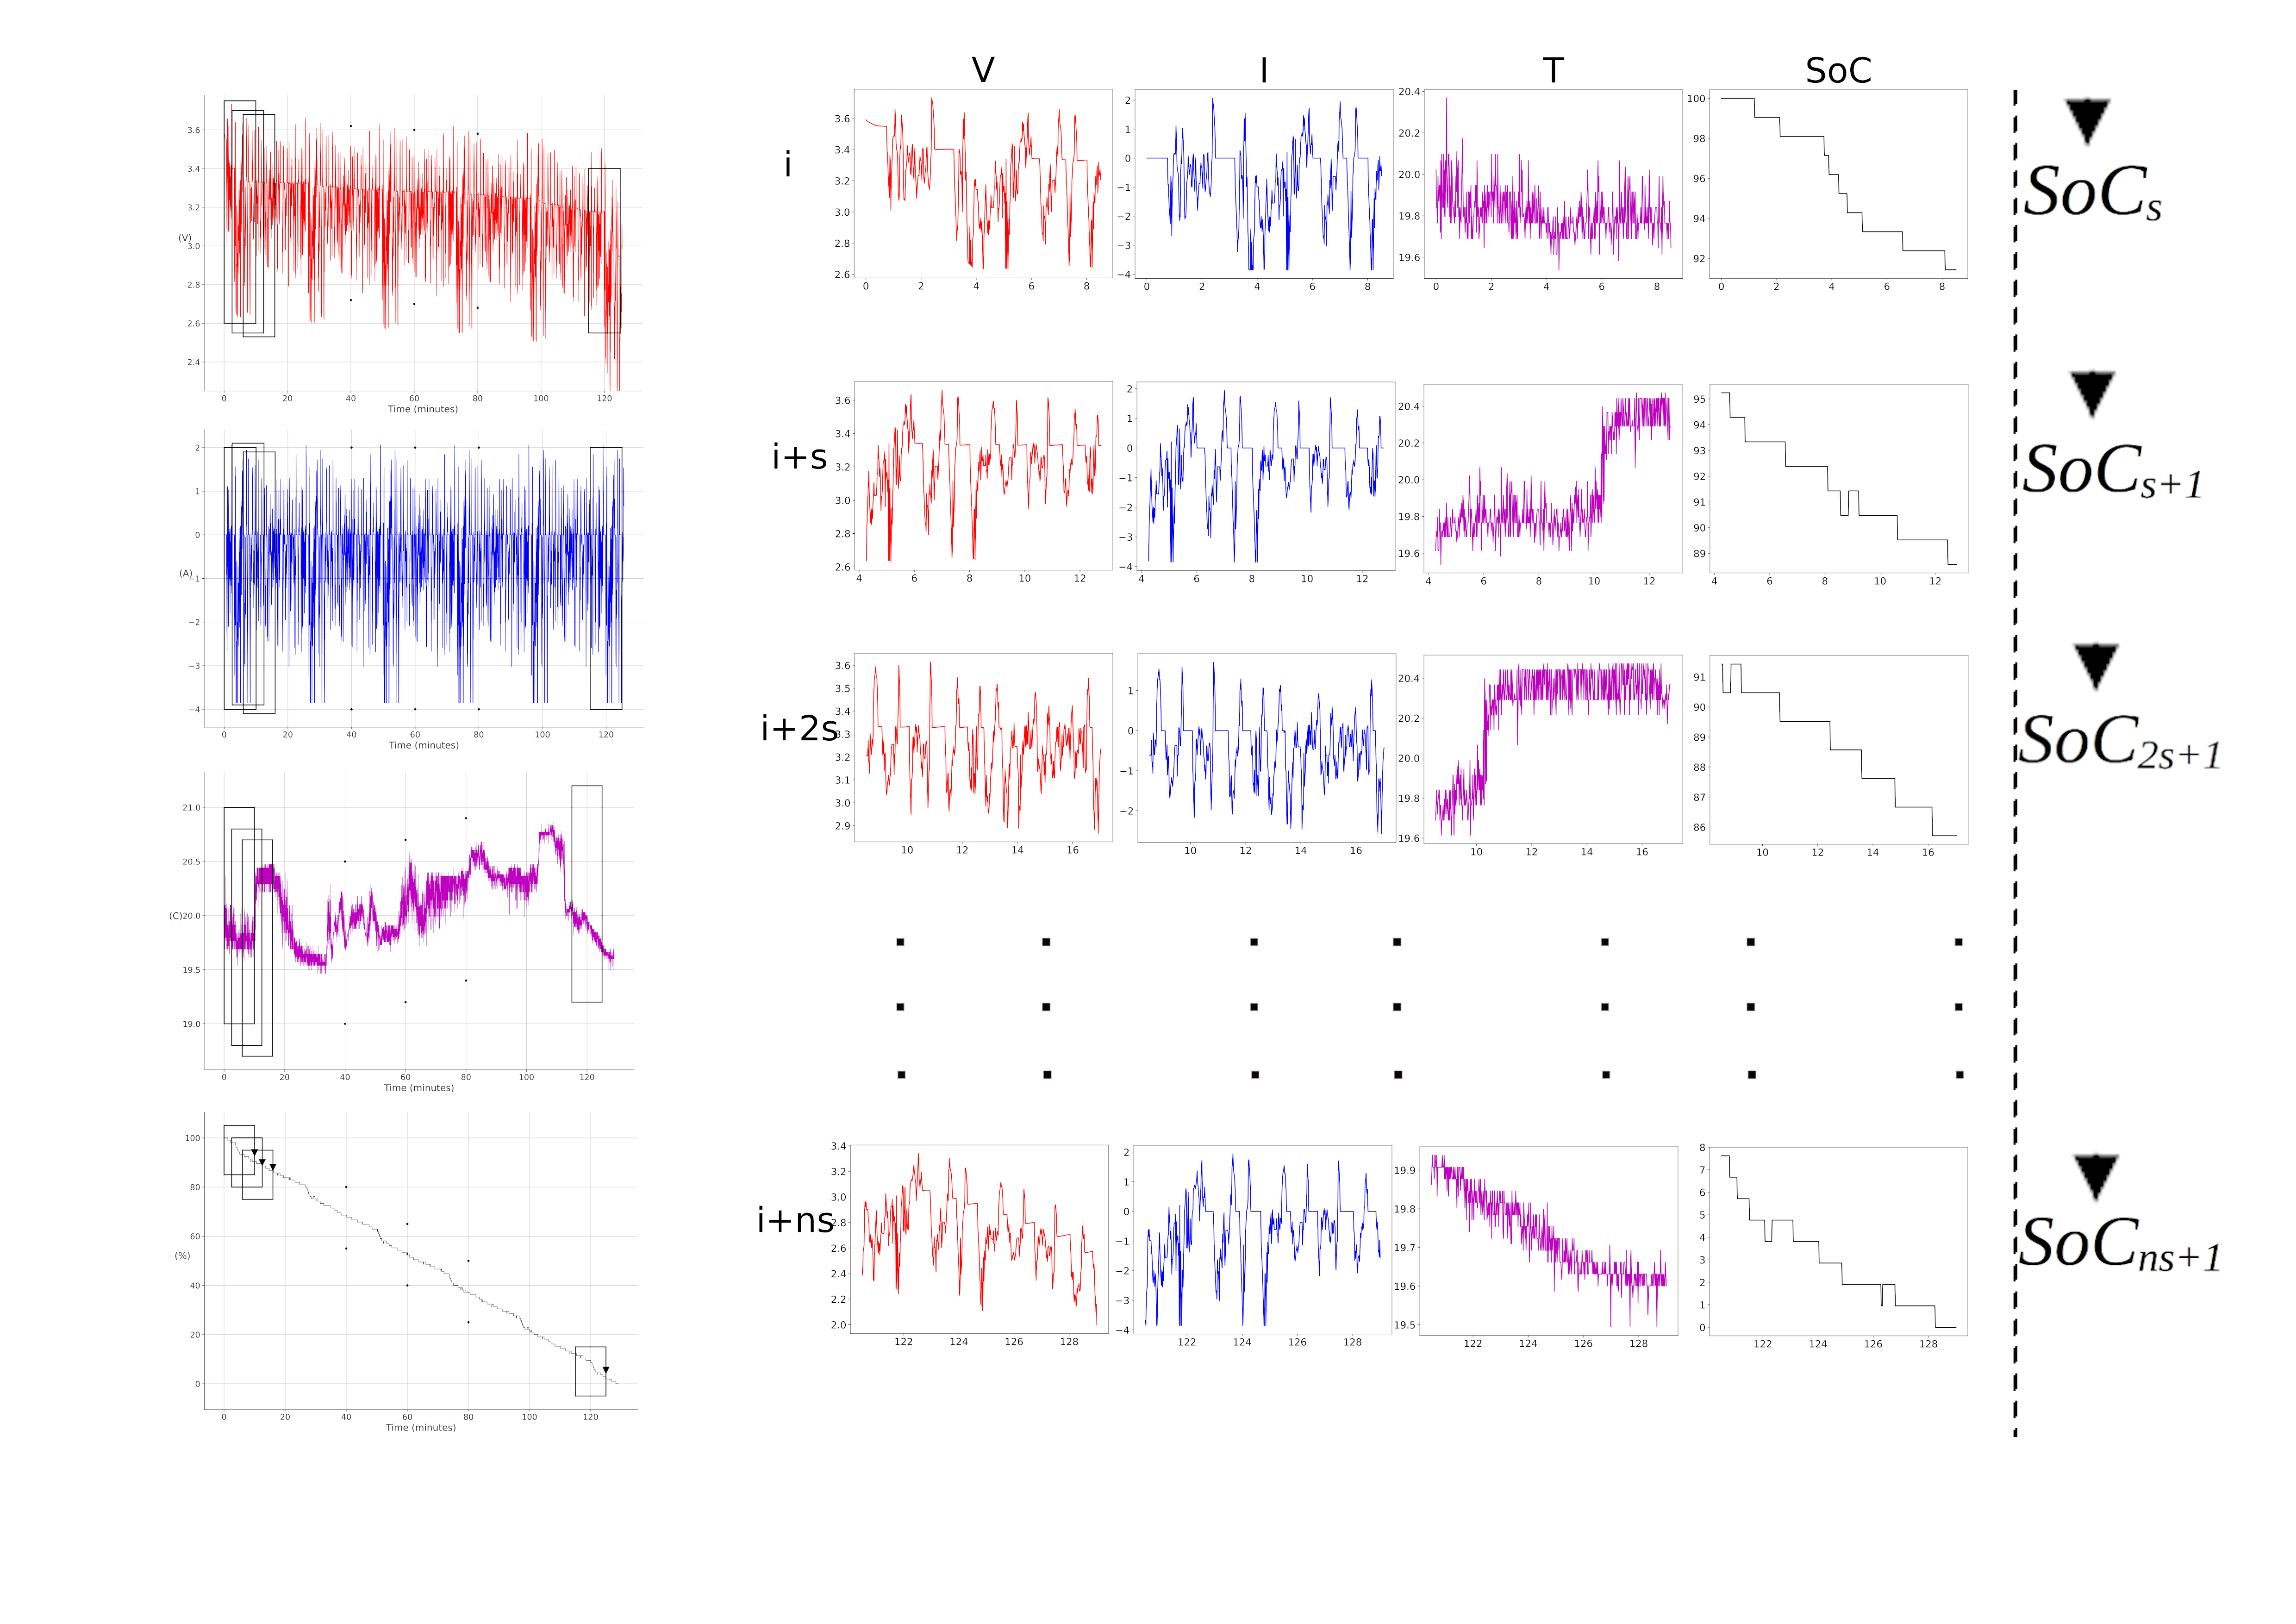
\includegraphics[width=0.9\linewidth]{II_Body/images/Windowing4f-A3.jpg}
        \caption{Data Windowing scheme. For visualisation purposes, the $s$-step has been used as $\sim 5$ minutes, which is different from actual implementation. Initial index $i$ was kept as a value close to the beginning of the data, around zero.}
        \label{fig:Windowing}
    \end{figure}
\end{landscape}